\documentclass{../iot-lecture}

\subtitle{I1820 Platforms}

\begin{document}

\begin{frame}
  \titlepage{}
\end{frame}
\begin{frame}
  \frametitle{Outline}
  \tableofcontents{}
\end{frame}

\section{Overview}

\begin{frame}
  \begin{figure}
    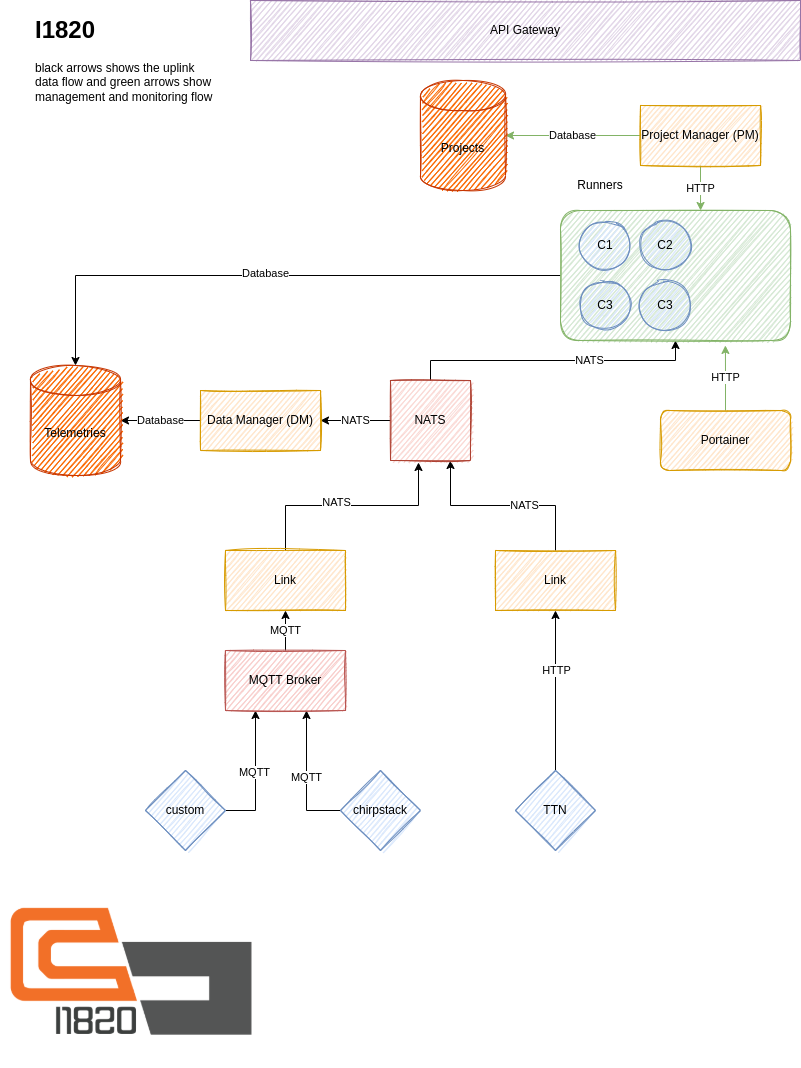
\includegraphics[height=\textheight]{./img/arch.png}
  \end{figure}
\end{frame}

\begin{frame}
  \frametitle{Features}
  \begin{itemize}
    \item Supports multiple interface for thing communications:
    \begin{itemize}
      \item HTTP
      \item MQTT
      \item LoRaWAN Integration through TTN
      \item LoRaWAN Integration through Chirpstack
    \end{itemize}
    \item Supports Application Integration by OpenAPI
    \item Microservice Architecture
    \item Users can define scenario to react based on events
    \item Users can define codecs to parse their data
  \end{itemize}
\end{frame}

\begin{frame}
  \frametitle{Link;\@ Uplink}
  \begin{itemize}
    \item Recieves data from HTTP or MQTT
    \begin{itemize}
      \item Based on pre-configured structure
      \item Supports Chirpstack and TTN for LoRaWAN
      \item Adding new structure or platforms required code change
    \end{itemize}
    \item Decodes data based on \textit{\color{LimeGreen} JSON}, \textit{\color{Orange} CBOR} or uses \textit{\color{RubineRed} custom decoder}
  \end{itemize}
\end{frame}

\begin{frame}
  \frametitle{PM;\@ The Project Manager}
  \begin{itemize}
    \item Builds projects and their {\color{Cyan} docker}
    \item Each project has a single docker node
    \item Manage and Monitor the docker node
  \end{itemize}
\end{frame}

\begin{frame}
  \frametitle{ElRunner;\@ Who runs in dockers}
  \begin{itemize}
    \item Runs scenario and decoders in Python
    \item Decodes if it isn't decoded with pre-written decoders
    \item Manage decoders and scenarios
  \end{itemize}
\end{frame}

\begin{frame}
  \frametitle{DM;\@ The Data Manger}
  \begin{itemize}
    \item Stores data into telemeteries database
    \item Pre-written queries
    \item Data aggregation
  \end{itemize}
\end{frame}

\begin{frame}
  \frametitle{API Sever}
  \begin{itemize}
    \item Manage Users and Permissions
    \item Manage Projects and their owners
    \item Payment
    \item \ldots
  \end{itemize}
\end{frame}

\end{document}
